\documentclass[titlepage]{article}

\usepackage[english]{babel}
\usepackage[utf8]{inputenc}
\usepackage{amsmath}
\usepackage{listings}
\usepackage{courier}
\usepackage{amsthm}
\usepackage{graphicx}
\usepackage[colorinlistoftodos]{todonotes}
\usepackage{amssymb}
\usepackage{mathtools}
\usepackage{listings}
\usepackage[inline]{enumitem}
\usepackage{tikz}
\usepackage{tabularx}
\usepackage{lstautogobble}
\usepackage{algorithm}
\usepackage{todonotes}
\usepackage[noend]{algpseudocode}
\usepackage[a4paper,left=3cm,right=3cm,top=3cm,bottom=3cm]{geometry}
\usepackage{titlesec}
\usepackage{siunitx}
\usepackage{mathrsfs}
\usepackage{setspace}
\usepackage{fixltx2e}
\usepackage{hyperref}
\usepackage{csquotes}
\usepackage{colortbl}
\usepackage{indentfirst}
\usepackage[T1]{fontenc}
\usepackage{float}
\usepackage{longtable}
\linespread{2}
\lstset{basicstyle=\footnotesize\ttfamily,breaklines=true,lineskip={-1pt}}
\titlelabel{\thetitle.\quad}
\allowdisplaybreaks
\delimitershortfall-1sp

\usetikzlibrary{arrows}
\usetikzlibrary{automata,positioning}

\title{Extend\\ Language Reference Manual}
\author{Ishaan Kolluri(isk2108), Kevin Ye(ky2294) Jared Samet(jss2272), Nigel Schuster(ns3158)}
\date{\today}
\begin{document}
\maketitle
\tableofcontents
\pagebreak
\section{Introduction to Extend}
	Extend is a domain-specific programming language used to designate ranges of cells as reusable functions. It abstracts dependencies between cells and models a dependency graph during compilation. In order to offer great performance for any size of datasets, Extend compiles down to LLVM.
	\newline
	Extend's syntax is meant to provide clear punctuation and easily understandable cell range access specifications, while maintaining the look of modern functional programming languages. Given Extend's functionality resonates well with spreadsheets, it borrows syntactical elements from programs such as Microsoft Excel.
\section{Structure of an Extend Program}
	Extend is predominantly composed of function declarations. In order to run the program, the \textbf{main} function will be executed. To illustrate the scope of the language, the OCaml grammar is attached below:
\lstinputlisting{./src/main/parser.mly}
\section{Types and Literals}
	\subsection{Primitive Data Types}
		Extend has two primitive data types, \textbf{numbers} and \textbf{ranges}. In the vein of Javascript, numbers are essentially 64-bit floating point numbers in Extend. Ranges are elaborated on in the next section. The user can choose to represent numbers in the following different ways:
		\newline
		\underline{\textbf{Char}}\newline
		A \textbf{char} literal is essentially a size 1 numerical range. At evaluation, the number in the range will be compared with its ASCII equivalent.
  		\newline
		\underline{\textbf{String}}\newline
  		A \textbf{string} literal is a range of numbers of size \textit{n}, where \textit{n} is the length of the string. The string 'hello' can be represented internally as [104, 101, 108, 108, 111].
		\newline
		\underline{\textbf{Integer}}\newline
		A \textbf{integer} can be represented as a size 1 numerical range as well. However, it retains its numerical value upon evaluation. 
		\newline
		\underline{\textbf{Float}}\newline
		A \textbf{float}, like Javascript numbers, can be represented as 64 bit, where the fraction is stored in bits 52 to 62.
		\newline
		Below is a snippet illustrating programmatic declarations for each of the above types.
  		\begin{lstlisting}
/* Integer */
num = 5;
/* Char */
chr = 'A'
/* String */
str = 'Hello'
/* Float */
num = 1.5;
  		\end{lstlisting}
	\subsection{Ranges}
		Ranges are a data type unique to the Extend language. It borrows conceptually from spreadsheets; a range is a group of cells with dimensions represented as rows and columns. Each range is either one or two-dimensional. A range is composed of cells, and cells are comprised of functions that can have dependencies on the values of other cells. 
		A range is written as follows:
		\begin{lstlisting}
/* This is a left-handed range, used to assign a value. */
[1,2]foo; /*Range with 1 row and 2 columns */
		\end{lstlisting}
		\subsubsection{Range Slicing}
			Extend somewhat mimics Python in its range slicing syntax; however, it offers the ability to slice a range in both absolute and relative terms.
			\begin{lstlisting}
foo[1,2] /* This evaluates to the cell value at row 1, column 2. */
foo[1,] /* Evaluates to the range of cells in row 1. */
foo[,2] /* Evaluates to the range of cells in column 2.*/
foo[,[1]] /* The internal brackets denote RELATIVE notation. 
In this case, 1 column right of the one currently being operated on. */ 
foo[5:, 7:] /* 5th row down, and 7th column from the absolute origin.
foo[[1:2], [5:7]] 
/* Selects the rows between the 1st and 2nd row from current row */
/* Selects the columns between 5th and 7th column from current column */
			\end{lstlisting}
		\subsubsection{The Underscore Symbol}
			The underscore(\_) symbol allows the dimension of the range to have an unspecified size. For example, in function signatures, using the underscore allows the return value to have various possible dimensions. An example is illustrated below:
			\begin{lstlisting}
[1,_]foo; 
/* A range with 1 row and an unknown, variable number of columns. */
			\end{lstlisting}

\section{Types and Literals}
		Extend has three primitive data types, \textbf{Number}, \textbf{String}, and \textbf{Empty}, and one composite type, \textbf{Range}.
	\subsection{Primitive Data Types}
		A \textbf{Number} is an immutable primitive value corresponding to a double-precision 64-bit binary format IEEE 754 value. Numbers can be written in an Extend source file as either integer or floating point constants; both are represented internally as floating-point values. There is no separate type representing an integer.

		A \textbf{String} is a immutable primitive value that is internally represented a C-style null-terminated byte array corresponding to ASCII values. A String can be written in an Extend source file as a sequence of characters enclosed in double quotes, with the usual escaping conventions. Extend does not allow for slicing of strings to access specific characters; access to the contents of a string will only be available through standard library functions.

		The \textbf{Empty} type can be written as the keyword \texttt{empty}, and serves a similar function to \texttt{NULL} in SQL; it represents the absence of a value.
		\newline
		\begin{table}[H]
		\centering
		\begin{tabular} {| l | l |}
			\hline
			\textbf{Primitive Data Types} & \textbf{Examples} \\ \hline
			Number & \texttt{42 or -5 or 2.71828 or 314159e-5} \\ \hline
			String & \texttt{"Hello, World!\textbackslash n" or "foo" or ""} \\ \hline
			Empty & \texttt{empty} \\ \hline
		\end{tabular}
		\end{table}
	\subsection{Ranges}
		Extend has one composite type, \textbf{Range}. A range is a subset of the cells of a variable, as described in section~\ref{sec:vardecl}. Ranges can be nested arbitrarily deeply and can be used to represent (immutable) lists, matrices, or more complicated data structures. For convenience, the range literal syntax can be used to implicitly declare an anonymous variable and assign the range to the entire contents of this variable.
\subsubsection{Range Literals}
		A range literal is a semicolon-delimited list of rows, enclosed in curly brackets. Each row is a comma-delimited list of numbers, strings, or range literals. A few examples follow:
		\lstinputlisting{./samples/legal_range_literals.xtnd}

\section{Expressions}
	Expressions in Extend allows for arithmetic and boolean operations, function calls, conditional branching,  extraction of contents of other variables, string concatenation, and determination of the location of the cell containing the expression. The sections for boolean and conditional operators refer to truthy and falsey values. The \texttt{Number} 0 is the only falsey value; all other values are truthy. As \texttt{empty} represents the absence of a value, it is neither truthy nor falsey.
	\pagebreak
		\subsection{Arithmetic Operators}
			The arithmetic operators listed below take one or two expressions and return a number, if both expressions are Numbers, or empty otherwise. Operators grouped within the same inner box have the same level of precedence, and are listed from highest precedence to lowest precedence. All of the binary operators are infix operators, and, with the exception of exponentiation, are left-associative. Exponentiation, bitwise negation, and unary negation are right-associative. All of the unary operators are prefix operators. The bitwise operators coerce their operands to signed 32-bit integers before performing the operation and evaluate to a Number.
			\begin{table}[H]
			\begin{tabular}{ |p{2cm}|p{3cm}|p{8cm}|  }
			\hline
			\textbf{Operator} & \textbf{Description} & \textbf{Definition} \\ \hline
			\rule{0pt}{3ex}\texttt{\~} & \texttt{Bitwise NOT } & {Performs a bitwise negation on the binary representation of an expression.} \\
			\rule{0pt}{3ex}\texttt{-} & \texttt{Unary negation} & {A simple negative sign to negate expressions.} \\ \hline
			\rule{0pt}{3ex}\texttt{**} & \texttt{Power} & {Returns the first expression raised to the power of the second expression} \\ \hline
			\texttt{*} & \texttt{Multiplication} & {Multiplies two expressions} \\
			\rule{0pt}{3ex}\texttt{/} & \texttt{Division} & {Divides first expression by second}. \\
			\rule{0pt}{3ex}\texttt{\%} & \texttt{Modulo} & {Finds the remainder by dividing the expression on the left side of the modulo by the right side expression.} \\
			\rule{0pt}{3ex}\texttt{<<} & \texttt{Left Shift} & {Performs a bitwise left shift on the binary representation of an expression.} \\
			\rule{0pt}{3ex}\texttt{>>} & \texttt{Right Shift} & {Performs a sign-propagating bitwise right shift on the binary representation of an expression.} \\
			\rule{0pt}{3ex}\texttt{\&} & \texttt{Bitwise AND} & {Performs a bitwise AND between two expressions.} \\ \hline
			\rule{0pt}{3ex}\texttt{+} & \texttt{Addition} & {Adds two expressions together.} \\
			\rule{0pt}{3ex}\texttt{-} & \texttt{Subtraction} & {Subtracts second expression from first.} \\
			\rule{0pt}{3ex}\texttt{|} & \texttt{Bitwise OR} & {Performs a bitwise OR between two expressions.} \\
			\rule{0pt}{3ex}\texttt{\^} & \texttt{Bitwise XOR} & {Performs a bitwise exclusive OR between two expressions.} \\ \hline
			\end{tabular}
			\end{table}
			\pagebreak
		\subsection{Boolean Operators}
			These operators take one or two expressions and evaluate to empty, 0 or 1. Operators grouped within the same inner box have the same level of precedence and are listed from highest precedence to lowest precedence. All of these operators besides logical negation are infix, left-associative operators. The logical AND and OR operators feature short-circuit evaluation. Logical NOT is a prefix, right-associative operator.
			\begin{table}[H]
			\begin{tabular}{ |p{2cm}|p{5cm}|p{7cm}|  }
			\hline
			\textbf{Operator} & \textbf{Description} & \textbf{Definition} \\ \hline
			\rule{0pt}{3ex}\texttt{!} & \texttt{Logical NOT} & {Evaluates to 0 or 1 given a truthy or falsey value respectively. \texttt{!empty} evaluates to \texttt{empty}.} \\ \hline
			\rule{0pt}{3ex}\texttt{==} & \texttt{Equals} & {Always evaluates to 0 if the two expressions have different types. If both expressions are primitive values, evaluates to 1 if they have the same type and the same value, or 0 otherwise. If both expressions are ranges, evaluates to 1 if the two ranges have the same dimensions and each cell of the first expression == the corresponding cell of the second expression.} \\
			\rule{0pt}{3ex}\texttt{!=} & \texttt{Not equals} & {\texttt{x != y} is equivalent to \texttt{!(x == y)}.} \\
			\rule{0pt}{3ex}\texttt{<} & \texttt{Less than} & {If the expressions are both Numbers or both Strings and the first expression is less than the first, evaluates to 1. If the expressions are both Numbers or both Strings and the first expression is greater than or equal to the first, evaluates to 0. Otherwise, evaluates to empty.} \\
			\rule{0pt}{3ex}\texttt{>} & \texttt{Greater than} & {Evaluates to 1 if the first expression is greater than the first; equivalent rules about typing as for \texttt{<}.} \\
			\rule{0pt}{3ex}\texttt{<=} & \texttt{Less than or equal to} & {Evaluates to 1 if the first expression is less than or equal to the second; equivalent rules about typing as for \texttt{<}.} \\
			\rule{0pt}{3ex}\texttt{>=} & \texttt{Greater than or equal to} & {Evaluates to 1 if the first expression is less than or equal to the second; equivalent rules about typing as for \texttt{<}.} \\ \hline
			\rule{0pt}{3ex}\texttt{\&\&} & \texttt{Short-circuit Logical AND} & {If the first expression is falsey or empty, evaluates to 0 or empty respectively. Otherwise, if the second expression is truthy, falsey, or empty, evaluates to 1, 0, or empty respectively.} \\ \hline
			\rule{0pt}{3ex}\texttt{||} & \texttt{Short-circuit Logical OR} & {If the first expression is truthy or empty, evaluates to 1 or empty respectively. Otherwise, if the second expression is truthy, falsey, or empty, evaluates to 1, 0, or empty respectively.} \\ \hline
			\end{tabular}
			\end{table}

\subsection{Conditional Expressions}
			There are two types of conditional expressions: a simple if-then-else expression written using the ternary operator \textbf{? :} and \texttt{switch} expressions which can represent more complex logic.

\subsubsection{Ternary Expressions}
\label{sec:Ternary}
A ternary expression, written as \texttt{cond-expr ? expr-if-true : expr-if-false} evaluates to \texttt{expr-if-true} if \texttt{cond-expr} is truthy, or \texttt{expr-if-false} if \texttt{cond-expr} is falsey. If \texttt{cond-expr} is empty, the expression evaluates to empty. Both expr-if-true and expr-if-false are mandatory. \texttt{expr-if-true} is only evaluated if \texttt{cond-expr} is truthy, and \texttt{expr-if-false} is only evaluated if \texttt{cond-expr} is falsey. If \texttt{cond-expr} is empty, neither expression is evaluated.

\subsubsection{Switch Expressions}
\label{sec:Switch}
A \texttt{switch} expression takes a optional condition, and a list of cases and expressions that the overall expression should evaluate to if the case applies. In the event that multiple cases are true, the expression of the first matching case encountered will be evaluated. An example is provided below:
\begin{lstlisting}
[1,1] foo := 3;
return switch (foo) {
	case 2: "foo is 2";
	case 3,4: "foo is 3 or 4";
	default: "none of the above";
}

/* Equivalently: */
return switch {
	case foo == 2:
		"foo is 2";
	case foo == 3, foo == 4:
		"foo is 3 or 4";
	default:
		"none of the above";
}
\end{lstlisting}
The format for a \texttt{switch} statement is the keyword \texttt{switch}, optionally followed by pair of parentheses containing an expression \texttt{switch-expr}, followed by a list of case clauses enclosed in curly braces and delimited by semicolons. A case clause consists of the keyword \texttt{case} followed by a comma-separated list of expressions \texttt{case-expr1 [, case-expr2, [...]]}, a colon, and an expression \texttt{match-expr}, or the keyword \texttt{default}, a colon, and an expression \texttt{default-expr}. If \texttt{switch-expr} is omitted, the value 1 is assumed. The \texttt{switch} expression evaluates to the \texttt{match-expr} for the first case where one of the \texttt{case-expr}s is truthy, if \texttt{switch-expr} is omitted, or equal (with equality defined as for the \texttt{==} operator) to \texttt{switch-expr}, if \texttt{switch-expr} is present, or \texttt{default-expr}, if none of the \texttt{case-expr}s apply.

The \texttt{switch} expression can be used to compactly represent what in most imperative languages would require a long string such as \texttt{if (cond1) \{...\} else if (cond2) \{...\}}. The \texttt{switch} operator is internally converted to an equivalent (possibly nested) ternary expression; as a result, it features short-circuit evaluation throughout.

\subsection {Additional Operators}
There are four additional operators available to determine the size and type of other expressions. In addition, the infix \texttt{+} operator is overloaded to perform string concatenation.
\begin{table}[H]
\begin{tabular}{ |p{2cm}|p{3cm}|p{8cm}|  }
\hline
\textbf{Operator} & \textbf{Description} & \textbf{Definition} \\ \hline
\texttt{size(expr)} & \texttt{Dimensions} & {Evaluates to a Range consisting of one row and two columns; the first cell contains the number of rows of \texttt{expr} and the second contains the number of columns. If \texttt{expr} is a Number, a String, or Empty, both cells will contain 1.} \\ \hline
\texttt{type(expr)} & \texttt{Value Type} & {Evaluates to "Number", "String", "Range", or "Empty".} \\ \hline
\texttt{row()} & \texttt{Row Location} & {No arguments; returns the row of the cell containing the formula} \\ \hline
\texttt{column()} & \texttt{Column Location} & {No arguments; returns the column of the cell containing the formula} \\ \hline
\texttt{+} & \texttt{String concatenation} & {"Hello, " + "World!\textbackslash n" == "Hello, World!\textbackslash n"}\\ \hline
\end{tabular}
\end{table}

\subsection {Function Calls}
A function expression consists of an identifier and an optional list of expressions enclosed in parentheses and separated by commas. The value of the expression is the result of applying the function to the arguments passed in as expressions. For more detail, see section~\ref{sec:Functions}.
\subsection{Range Expressions}
Range expressions are used to select part or all of a range. A range expression consists of a bare identifier, a bare range literal, or an expression and a selector. If a range expression has exactly 1 row and 1 column, the value of the expression is the value of the single cell of the range. If it has more than 1 row or more than 1 column, the value of the expression is the selected range. If the range has zero or fewer rows or zero or fewer columns, the value of the expression is \texttt{empty}. If a range expression with a selector would access a row index or column index greater than the number of rows or columns of the range, or a negative row or column index, the value of the expression is \texttt{empty}.
\subsubsection{Slices}
A slice consists of an optional integer literal or expression \texttt{start}, a colon, and an optional integer literal or expression \texttt{end}, or a single integer literal or expression \texttt{index}. If \texttt{start} is omitted, it defaults to 0. If \texttt{end} is omitted, it defaults to the length of the dimension. A single \texttt{index} with no colon is equivalent to \texttt{index:index+1}. Enclosing \texttt{start} or \texttt{end} in square brackets is equivalent to the expression \texttt{row() + start} or \texttt{row() + end}, for a row slice, or \texttt{column() + start} or \texttt{column() + end} for a column slice. The slice includes \texttt{start} and excludes \texttt{end}, so the length of a slice is \texttt{end - start}. A negative value is interpreted as the length of the dimension minus the value.
			As mentioned above, the value of a range that is not 1 by 1 is a range, but the value of a 1 by 1 range is essentially dereferenced to the result of the cell formula.
\subsubsection{Selections}
A selection expression consists of an expression and a pair of slices separated by a comma and enclosed in square brackets, i.e. {[}\texttt{row\_slice, column\_slice}{]}. It can also be written as the hash symbol \texttt{\#} and an expression. As mentioned earlier, the composite \textbf{range} type has the ability to slice in both an absolute and relative fashion. If one of the dimensions of the range has length 1, the comma and the slice for that dimension can be omitted. If the comma is present but a slice is omitted, that slice defaults to {[}\texttt{0}{]} for a slice corresponding to a dimension of length greater than one, or \texttt{0} for a slice corresponding to a dimension of length one.
\subsubsection{Corresponding Cell}
A very common selection to make is the cell in the "corresponding location" of a different variable. Since this case is so common, \texttt{\#var}
is syntactic sugar for \texttt{var{[},{]}}. As a result, if \texttt{var} has more than column and more than one row, \texttt{\#var} is equivalent to \texttt{var{[}row(),column(){]}}. If \texttt{var} has multiple rows and one column, it is equivalent to \texttt{var{[}row(),0{]}}. If \texttt{var} has one row and multiple columns, it is equivalent to \texttt{var{[}0,column(){]}}; and if \texttt{var} has one row and one column, it is equal to \texttt{var{[}0,0{]}}.

\subsubsection{Selection Examples}
\begin{lstlisting}
foo[1,2] /* This evaluates to the cell value in the second row and third column. */
foo[1,:] /* Evaluates to the range of cells in the second row of foo. */
foo[:,2] /* Evaluates to the range of cells in the third column of foo. */
foo[:,[1]] /* The internal brackets denote RELATIVE notation.
In this case, 1 column right of the column of the left-hand-side cell. */

foo[1,] /* Equivalent to foo[1,[0]] if foo has more than one column
or foo[1,0] if foo has one column */

foo[5:, 7:] /* All cells starting from the 6th row and 8th column to the bottom right */

foo[[1:2], [5:7]]
/* Selects the rows between the 1st and 2nd row after LHS row, and
   between 5th and 7th column from LHS column */

/* In this example, each cell of bar would be equal to the cell
 * in foo in the equivalent location plus 1. */
[5,5] foo;
[5,5] bar := #foo + 1; // #foo = foo[[0],[0]]

/* In this example, bar would be a 3x5 range where in each row,
 * the value in bar is equal to the value in foo in the same column.
 * In other words, each row of bar would be a copy of foo. */
[1,5] foo; // foo has 1 row, 5 columns
[3,5] bar := #foo; // #foo = foo[0,[0]]

/* In this example, the values of baz would be
 * 11, 12, 13 in the first row;
 * 21, 22, 23 in the second row;
 * 31, 32, 33 in the third row. */
foo := {1,2,3}; // 1 row, 3 columns
bar := {10;20;30}; // 3 rows, 1 column
[3,3] baz := #foo + #bar; // Equivalent to foo[0,[0]] + bar[[0],0]

\end{lstlisting}
\subsection{Precedence Expressions}
A precedence expression is used to force the evaluation of one expression before another, when that order of operation is required for functions with side-effects. It consists of an expression \texttt{prec-expr}, the precedence operator \texttt{->}, and an expression \texttt{succ-expr}. The value of the expression is \texttt{succ-expr}, but the value of \texttt{prec-expr} will be calculated first and the result ignored. All functions written purely in Extend are free of side effects. However, some of the external functions provided by the standard library, such as for file I/O and plotting, do have side effects.

\section{Functions}
\label{sec:Functions}
Functions lie at Extend's core; however, they are not \textit{first class objects}. Since it can be verbose to write certain operations in Extend, the language will feature a small number of built-in functions and and a comprehensive standard library. An important set of built-in functions will handle I/O (see section~\ref{sec:IO}). Besides the built-in file I/O functions, all functions in Extend are free of side effects.
\subsection{Format}
\label{sec:funcdecl}
Every function in Extend follows the same format, but allows some optional declarations. As in most programming languages, the header of the function declares the parameters it accepts and the dimensions of the return value. The body of the function consists of an optional set of variable declarations and formula assignments, which can occur in any order, and a return statement, which must be the last statement in the function body. All variable declarations and formula assignments, in addition to the return statement, must be terminated by a semicolon.
This very simple function returns whatever value is passed into it:
\lstinputlisting{./samples/functions_simple.xtnd}
The leading \texttt{[1,1]} marks the return dimensions. \texttt{foo} is the function name. In parentheses the function arguments are declared, again with dimensions of the input. The body of the function follows, which in this case is only the return statement.
\subsection{Variable Declaration}
\label{sec:vardecl}
A variable declaration associates an identifier with a range of the specified dimensions, which are listed in square brackets before the identifier. For convenience, if the square brackets and dimensions are omitted, the identifier will be associated with a 1x1 range, and if only a single dimension is listed instead of two, the identifier will be associated with a range consisting of one row and the specified number of columns. In addition, multiple identifiers, separated by commas, can be listed after the dimensions; all of these identifiers will be separate ranges, but with equal dimension sizes. The dimensions can be specified either as literal integers or as expressions that evaluate to integers.
\begin{lstlisting}
[2, 5] foo; // Declares foo as a range with 2 rows and 5 columns
[m, n] bar; // Declares bar as a range with m rows and n columns
baz; // Declares baz as a 1x1 range
[10] ham, eggs, spam; // Declares ham, eggs and spam as distinct 1x10 ranges
\end{lstlisting}
\subsection{Formula Assignment}
\label{sec:formula}
A formula assignment assigns an expression to a subset of the cells of a variable. Unlike most imperative languages, this expression is not immediately evaluated, but is instead only evaluated if and when it is needed to calculate the return value of the function. A formula assignment consists of an identifier, an optional pair of slices enclosed in square brackets specifying the subset of the cells that the assignment applies to, an \texttt{=}, and an expression, followed by a semicolon. The slices specifying the cell subset can contain arbitrary expressions, as long as the expression taken as a whole evaluates to an integer.
\begin{lstlisting}
[5, 2] foo, bar;
foo[0,0] = 42; // Assigns the expression 42 to the first cell of the first row of foo
foo[0,1] = foo[0,0] * 2; // Assigns (foo[0,0] * 2) to the 2nd cell of the 1st row of foo
bar = 3.14159; // Assigns pi to every cell of every row of bar

/* The next line assigns foo[[-1],0] + 1 to every cell in
   both columns of foo, besides the first row */
foo[1:,0:1] = foo[[-1],0] + 2;
\end{lstlisting}
The last line of the source snippet above demonstrates the idiomatic Extend way of simulating an imperative language's loop; foo[4,0] would evaluate to 42+2+2+2+2 = 50 and foo[4,1] would evaluate to (42*2)+2+2+2+2 = 92. Although this may appear wasteful, intermediate values can be garbage collected once they are no longer needed to calculate the function's return value.
\subsubsection{Combined Variable Declaration and Formula Assignment}
For convenience, a variable declaration and a formula assignment to all cells of that variable can be combined on a single line by inserting a \texttt{:=} and an expression after the identifier. Multiple variables and assignments, separated by commas, can be declared on a single line as well.
\begin{lstlisting}
/* Creates two 2x2 ranges; every cell of foo evaluates to 1 and every cell of
   bar evaluates to 2. */
[2,2] foo := 1, bar := 2;
\end{lstlisting}
\subsubsection{Formula Assignment Errors}
If the developer writes code in such a way that more than one formula applies to a cell, this causes a compile-time error if the compiler can detect it or a runtime error if the compiler cannot detect it in advance and the cell is evaluated. If there is no formula assigned to a cell, the cell will evaluate to \texttt{empty}.
\subsection{Dimension Assignment}
\par Extend will feature gradual typing for function declarations. This will enable users with a weak experience in typing to use the language, while allowing more sophisticated developers to enforce type checking at compile time. In addition, it allows the developer to return ranges whose size is an unpredictable or complex function of the inputs.
\par To avoid specifying the precise return dimensions, an underscore can be used. This marks a variable range. Thus our function now looks like this:
\lstinputlisting{./samples/functions_dim_range_u.xtnd}
Here we are selecting a range from arg1 that depends on the value of arg2 and can therefore not be known ahead of time.
\subsection{Parameter Declarations}
If a parameter is declared with an identifier for the dimensions, instead of an integer literal, that identifier will contain the dimension size of the argument inside the function. In addition, expressions consisting solely of other identifiers are allowed, and will cause a run-time error if the sizes of the arguments are not consistent.
\par However Extend will feature even more options to specify ranges. If a certain operation should be applied to a range of numbers of unknown size, the size can be inferred at runtime and match the return size:
\lstinputlisting{./samples/functions_dim_range_v.xtnd}
This function will add 1 to each element in arg. Notice, that \texttt{m} is used across the function as a variable identifier to apply the operation to the range.
\par Summarizing, we have 3 ways of specifying a return range:\newline
\begin{tabularx}{\columnwidth}{| c | c | X |} \hline
Type & Symbol Example & Description \\ \hline
Number & 3 & A number is the simplest descriptor. It specifies the absolute return size \\ \hline
Expression & bar * 2 & An expression that can be anything, ranging from a simple arithmetic operation to a function call. To use this, any identifier used, must also be present as a range descriptor in a function parameter. \\ \hline
Underscore & \_ & This marker is unique, since it is a wildcard. While the other options aim to be specific, the underscore circumvents declaring the range size. \\ \hline
\end{tabularx}
\subsection{Application on Ranges}
Extend gives the developer the power to easily apply operations in a functional style on ranges. As outlined in the section above, there are various ways to apply functions to ranges. A feature unique to Extend is the powerful operation on values and ranges. To apply a function on a per cell basis, the corresponding variable needs to be preceded by "\#". The following function applies cell wise addition:
\lstinputlisting{./samples/functions_range_single.xtnd}
While both function above result in the same value, and only show the syntactical difference. If we wanted each cell to to be the square root divided by the sum of the input we have the following:
\lstinputlisting{./samples/functions_range_mix.xtnd}
Notice that \texttt{arg} is only once preceded by \texttt{\#}.
\subsection{Dependencies Illustrated}
The dependency resolution is another asset that sets Extend apart from other languages. Most languages compile ordinarily and execute the given commands sequentially. Extend builds a dependency graph. The advantage of this is that only relevant code segments will be executed. Given the function
\lstinputlisting{./samples/functions_dep_graph.xtnd}
The dependency graph will look like this: \newline
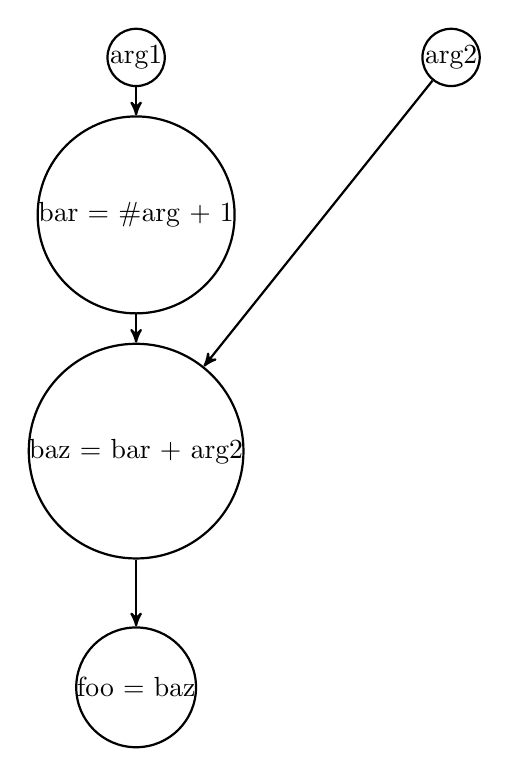
\begin{tikzpicture}[->,>=stealth',shorten >=0pt,auto,node distance=3cm,
        thick,main/.style={circle,draw,minimum size=0.6cm,inner sep=0pt]}]
		\node [main] (1) at (0, 2) {arg1};
		\node [main] (2) at (4, 2) {arg2};
		\node [main] (3) at (0, 0) {bar = \#arg + 1};
		\node [main] (4) at (0, -3) {baz = bar + arg2};
		\node [main] (5) at (0, -6) {foo = baz};
		\draw (1) to (3);
		\draw (3) to (4);
		\draw (4) to (5);
		\draw (2) to (4);
\end{tikzpicture} \newline
Notice that \texttt{faz} does not appear in the graph, because it is not relevant for the return value. Ultimately this graph enables Extend to find the leaves, evaluate code paths in the best configuration and even in parallel.

\section{Standard Library Reference}

\subsection{File I/O}
\begin{lstlisting}
open(filename, mode) - returns a file handle for use with the other file I/O functions
close(file_handle) - close a file handle
read(file_handle, num_bytes) - reads num_bytes from a file; 0 reads entire file
readline(file_handle) - read until the first newline
write(file_handle, buffer) - write the contents of buffer (a String) to the handle
STDIN, STDOUT, STDERR - global variables initialized to the file handles associated with stdin, stderr, and stdout
print_endline(val) - convert val to a string and write to STDOUT
\end{lstlisting}

\subsection{Math Functions - Imported straight from C}
\begin{lstlisting}
sin(x), cos(x), tan(x), acos(x), asin(x), atan(x), sinh(x), cosh(x), tanh(x),
exp(x), log(x), log10(x), sqrt(x), ceil(x), fabs(x), floor(x), isNaN(x)
random() - Just for fun - very non-random.
\end{lstlisting}

\subsection{Math Functions - Not imported from C}
\begin{lstlisting}
isInfinite(x) - returns -1 for -infinity, 0 for finite, or 1 for +infinity
round(val, number_of_digits);
gcd(m, n) - returns the GCD of two numbers
lcm(m, n) - returns the LCM of two numbers
sign(arg) - returns -1, 0, or 1
sum(rng) - adds all the numbers in rng
nmax(n1, n2) - returns the max of two numbers
max(rng) - returns the largest number in a range
nmin(n1, n2) - returns the min of two numbers
min(rng) - returns the smallest number in a range
avg([m,n] rng) - return the average of the numbers in a range
stdev([m,n] rng) - return the standard deviation of the numbers in a range
sumsq(rng) - returns the sum of the squares of the numbers in rng
sumproduct([m,n] rng1, [m,n] rng2) - returns the inner product of rng1 and rng2
sumxmy2([m,n] rng1, [m,n] rng2) - returns the sum of squared differences between the elements of rng1 and rng2
mmult([m,n] rng1, [n,p] rng2) - multiplies two matrices
linest([p,q] known_ys, [p,q] known_xs) - performs a linear regression with known_ys as the dependent variables and known_xs as the independent variables
normalize([m,n] arg) - return the unit norm vector in the same direction as arg
\end{lstlisting}

\subsection{String Functions}
\begin{lstlisting}
len(str) - returns the length of a String
toASCII(val) - returns a 1 x n range of the ASCII values of a String
fromASCII(val) - converts a 1 x n range of ASCII values into a String
parseFloat(str) - wrapper around C atof()
toUpper(text) - converts a string to uppercase
toLower(text) - converts a string to lowercase
left(str, num_chars) - returns the leftmost num_chars of str
right(str, num_chars) - returns the rightmost num_chars of str
substring(str, start, length) - returns a substring of str
repeat(str, num) - repeat a string, num times.
toString(arg) - convert any value into a String representation
ltrim(s) - remove whitespace at the beginning of s
rtrim(s) - remove whitespace at the end of s
trim(s) - remove whitespace on both ends of s
reverse(s) - reverses a string
padLeft(str, pad_char, total_length) - for a string shorter than total_length, pad on the left with pad_char
charAt(str, i) - return the ASCII code of the ith character of str
parseString(s) - best efforts to convert a string into the correct value
\end{lstlisting}

\subsection{Plotting}
\begin{lstlisting}
bar_chart(file_handle, labels, vals);
line_chart(file_handle, labels, x_vals);
\end{lstlisting}

\subsection{Range Functions}
\begin{lstlisting}
transpose([m,n] rng) - transpose a matrix; works with any dimensions
flatten([m,n] rng) - turn a rectangular range into a long row vector
isNumber(x) - equal to typeof(x) == "Number"
isEmpty(x) - equal to typeof(x) == "Number"
colRange(start, end) - return a column vector with the integers from start to (end-1)
rowRange(start, end) - return a row vector with the integers from start to (end-1)
match(list, val) - finds the first occurence of val in list; list can be either a row or a column vector and does not need to be sorted
bsearch(list, val) - finds the first occurrence of val in list; list must be a sorted column vector
join([m,n] cells, joiner) - concatenate the string representation of either a column or a row vector, using joiner as the delimiter
joinRange([m,n] cells, rowJoiner, colJoiner) - concatenate a range, joining rows with rowJoiner and columns with colJoiner
numRows(arg) - return the number of rows in arg
numCols(arg) - return the number of columns in arg
split(string, splitter) - returns a row vector of strings using splitter (which must be a one-character String) as a delimiter
splitToRange(string, row_splitter, col_splitter) - returns a range of strings using row_splitter as the row delimiter and col_splitter as the column delimiter
    case charAt(trimmed,0) == toASCII("{") && charAt(trimmed,-1) == toASCII("}"):
append([m,n] rg1, [p,q] rg2) - concatenate two ranges, horizontally
stack(rg1, rg2) - concatenate two ranges, vertically
mergesort([m,n] rng, sort_col) - return a sorted copy of rng, using sort_col for comparisons
\end{lstlisting}

\section{Example Program}
\lstinputlisting{./samples/sequence.xtnd}

\end{document}
